\documentclass[uplatex]{jsarticle}
\AtBeginDvi{\special{pdf:mapfile dlbase14.map}}
\usepackage[dvipdfmx]{graphicx}
\usepackage{ascmac}
\usepackage{url}
\usepackage{plext}
\usepackage{listings,jlisting}

\lstset{language=c,%
  basicstyle=\ttfamily\scriptsize,%
  commentstyle=\textit,%
  classoffset=1,%
  keywordstyle=\bfseries,%
  frame=tRBl,%
  framesep=5pt,%
  showstringspaces=false,%
  numbers=left,%
  stepnumber=1,%
  numberstyle=\tiny,%
  tabsize=2%
}
\begin{document}

\title{EDAツールを用いた論理回路設計}
\author{名古屋大学工学部電気電子・情報工学科情報コース\\酒井 英伸(学籍番号081330766)\\sakai.hidenobu@f.mbox.nagoya-u.ac.jp}
\date{2016/10/6, 13}
\maketitle

\tableofcontents


\clearpage
%===================================================================
\section{はじめに}
%===================================================================

今回の実験では、ハードウェア記述言語であるVerilog HDLを用いて、設計を行う。また、そのコードの機能レベルの
シミュレーションや論理合成をソフトウェア上で行い、回路の動作検証、評価は実験1に関しては、書き換え可能な論理素子
であるFPGA(Field Programmable Gate Array)を使用した。

%===================================================================
\section{2入力1出力セレクタ回路の設計と動作実験(実験1)}
%===================================================================

%---------------------------------------------------------------------
\subsection{目的・概要}
%---------------------------------------------------------------------

この実験では、2入力1出力セレクタ回路の回路の設計と動作実験を行う。また、その機能レベルシミュレーションや
論理合成を行うための環境設定や、ソフトウェアの使い方を理解するとともに、書き換え可能な論理素子であるFPGA
を搭載した実験基盤を用いて、FPGA上に設計した回路を実現することを目的とする。。

%---------------------------------------------------------------------
\subsection{実験手順}
%---------------------------------------------------------------------

はじめに、以下の手順で今回の実験を行うためのコンピュータの環境は以下のとおりである。

\begin{itemize}
  \item OS: Linux
  \item Kernel: 2.6.32-642.6.1.el6.x86\_64
\end{itemize}

%----------------------------------
\subsubsection{EDAツールの環境設定}
%----------------------------------

\begin{enumerate}
  \item
    端末上で「{\tt ln -s /pub1/jikken/eda3/cadsetup.csh.altera path/to/directory}」
    \fontnote{lnコマンドはファイルやディレクトリへのリンクを作成するコマンド.}
    と入力して、ファイルのシンボリックリンク
    \fontnote{lnコマンドに-sオプションを指定することで、作成される。特定のファイルやディレクトリを指し示す別のファイルを作成して、それを通じて本体を三章できるようにする仕組みのこと.}
    を自分の作業用のディレクトリに作成した。
  \item 
    作成した設定ファイルを読み込むために「\tt source /path/to/directory/cadsetup.csh.altera}」
    \footnote{指定したファイルを読み込む.}
    と入力した。(この操作は端末を起動する度に実行する。)
\end{enumerate}

%----------------------------------
\subsubsection{Verilog HDLによる回路記述}
%----------------------------------

今回の実験では図\ref{fig:1}のような2入力1出力セレクタ回路を設計した。
仕様は以下の通りであった。

\begin{itemize}
  \item 入力: データD0, D1(それぞれ1ビット), セレクト信号S1(1ビット)
  \item 出力: データY(1ビット)
  \item 機能: セレクト信号S1の値が0か1かにより、データD0, D1の値をYに出力
  \item 図\ref{fig:1}はこのセレクタ回路の回路図と真理値表である。
\end{itemize}

\begin{figure}[htb]
  \begin{center}
    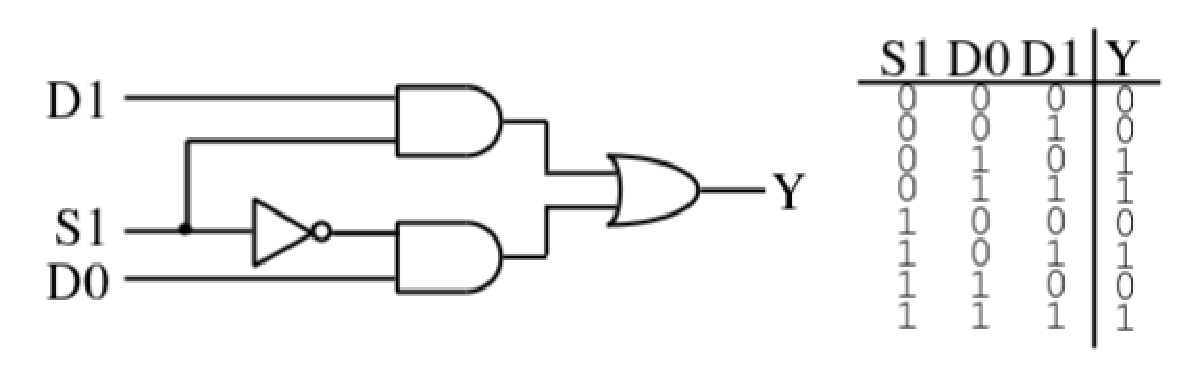
\includegraphics[width=13cm]{images/fig01.eps}
    \caption{2入力1出力セレクタ回路の回路図と真理値表}
    \label{fig:01}
  \end{center}
\end{figure}

まずは、2入力1セレクタ回路の記述を行った。
ソースコードは以下のようになった。

\lstinputlisting[caption=セレクタ回路,label=mux21.v]{../../jikken1/mux21.v}

このコードの説明を以下に記述する。

\begin{itemize}
  \item 1~5行目はコメントである。
  \item VerilogHDLでは、モジュールで一つの回路を記述するため、{\tt module ... endmodule}という記述をした。
  \item 7行目でモジュール名{\tt mux21} を定義して、ポート(入出力インタフェース)を( ... )内に記述した。
  \item 8, 9行目で各ポートの型(入力、出力、ビット数)を宣言した。
  \item 11行目は12行目の式のコメントである。
  \item 
    12行目で{\tt assign}文で、出力Yに論理式$(\lnot S_1 \land D_0) \lor (S_1 \land D_1)$を対応させた。この論理式は、図\ref{fig:1}の真理値表に対応している。
    {\tt assign}文は、シミュレーションの最中に、右辺のオブジェクトの値に変化が生じる度に実行される。
\end{itemize}

回路の設計をするには回路そのもの記述の他に、その記述した回路が正しく動作するかのテストの記述が必要となる。
これをテストベンチといい、今回の{\tt mux21.v}も同様にセレクタ回路の動作を確認するためのテストベンチ、{\tt test\_mux21.v}を作成した。

\lstinputlisting[caption=セレクタ回路のテストベンチ,label=test_mux21.v]{../../jikken1/test_mux21.v}

このコードも同様に説明を以下に記述する。   

\begin{itemize}
  \item 1~4行目はコメントである。
  \item 6行目で、シミュレーションの単位時間と精度を宣言した。今回はどちらも1nsと宣言した。
  \item 7行目で、mux21.vを取り込む記述をした。
  \item 9行目の {\tt module}以降で、テストベンチモジュールの宣言を行っている。
  \item 12行目で信号を与える入力ポートを指定した。
        {\tt reg}は記憶素子を表すオブジェクトである。
  \item 15行目で信号値を観測する出力ポートを指定した。
        {\tt wire}は配線を表すオブジェクトで、下位階層の出力ポートに接続しているオブジェクトを{\tt wire}宣言する。
  \item 20行目 ~ 34行目でテストパタンを宣言した。
        このテストパタンでは送る信号を表\ref{tab:1}にまとめた。また、図\ref{fig:1}の真理値表に基づいて、予想される出力Yの値も記述した。
\end{itemize}

\begin{table}[htb]
  \begin{center}
    \caption{test\_mux21.vによるテストパタン}
    \begin{tabular}{c|ccc|c} \hline
            & S1 & D0 & D1 & 予想される出力Y \\ \hline \hline
      初期値   & 0 & 0 & 0 & 0 \\
      20ns後  & 0 & 1 & 0 & 1 \\
      40ns後  & 1 & 1 & 0 & 0 \\
      60ns後  & 0 & 0 & 0 & 0 \\
      160ns後 & \multicolumn{3}{c|}{終了} & 0 \\ \hline
    \end{tabular}
    \label{tab:1}
  \end{center}
\end{table}

%----------------------------------
\subsubsection{機能レベルシミュレーション}
%----------------------------------

Verilog HDLで記述した回路が,機能的に正しく動作するかどうかを調べるために,論理シミュレータを用いた。
論理シミュレータには,Altera社のModelSim version 10.1d を用いた。
以下の手順で機能レベルシミュレーションを行った。

\begin{enumerate}
  \item 「{\tt vsim test\_mux21.v &}」コマンドを端末上で実行して、ModelSimでtest\_mux21.vを開いた。
  \item ModelSimのコンソールで「{\tt vlib work}」を実行して、ライブラリを作成した。
  \item 
    次に、「{\tt vlog test\_mux21.v}」コマンドを実行して、VerilogHDLで記述されたファイルのコンパイルを行った。
    この時、コンソール上で正しくコンパイルできた場合に表示される「{\tt Top level modules: test}」というメッセージを確認した。
  \item 最上位モジュールを読み込むために「{\tt vsim test}」を十個浮いて、コンパイルしたVerilogHDL記述内の最上位モジュールを読み込む。
  \item 次に、波形ウィンドウを「{\tt view wave}」コマンドで表示して、全ての入出力ポートの波形を表示する設定を「{\tt add wave *}」コマンドで行った。
  \item 最後に「{\tt run 80ns}」とコンソールに入力して、シミュレーションを開始し、その結果の波形を得た。
\end{enumerate}

%----------------------------------
\subsubsection{論理合成}
%----------------------------------

論理合成で、ハードウェア記述言語によって記述された回路を最適化して、ゲートレベルの記述であるネットリストに変換する。
論理合成には、FPGA設計フローにおける論理合成からFPGAマッピングまでの機能をサポートしているFPGA用統合開発ソフトウェアの
Quartus II Web Edition version 13.0.1を用いた。以下の手順で論理合成を行った。

\begin{enumerate}
  \item あらかじめ情報工学部実験用のサイトに上がっていたmux21.qpfをダウンロードした。
  \item 端末から「{\tt quartus &}」を実行してQuartus IIを起動して、プロジェクトファイルmux21.qpfを開いた。
        この時、Project Navigator1ウィンドウのEntity部分にコンパイル対象のFPGAとモジュールの名称(mux21~が表示されていることを確認した。
  \item ProcessingタブのStart Compilationでコンパイルを実行した。コンパイルが完了されると、メッセージウィンドウが開いてエラーが表示されていないことを確認した。
  \item コンパイル結果の確認を行った。Technology Map Viewerを用いて、咲いて季語の回路構成の確認や、Flow Summaryのロジックエレメントの確認をした。
        また、TImeQuest Timing Analyzerを用いて回路の遅延時間を確認した。
\end{enumerate}

%----------------------------------
\subsubsection{FPGAボードでの動作実験}
%----------------------------------

機能レベルシミュレーション、論理合成を行ったので、FPGAマッピングをするために、端末上で論理合成、レイアウト、FPGAマッピングの各機能を実行する一連の処理をまとめて実行した。
こkでのコンパイルはCUIで行い、「{\tt Quartus II Full Compilation was successful.}」と表示され、コンパイルが成功していることを確認した。
また、ディレクトリにmux.sofが生成されていることを確認した。

次に、以下の手順でAltera DE2-115ボードにsofファイルをインストールした。

\begin{enumerate}
  \item DE2-115ボードのマシンをUSBケーブルで接続した。また、DE2-115ボードに電源を入れるために電源を供給する専用のACアダプタを接続して、電源を入れた。
  \item 端末で「{\tt dmesg}」と入力して、マシンがボードを認識していることを確認した。
  \item ダウンロード用の設定ファイルmux21.cdfを作業ディレクトリに置いて、端末で「{\tt quartus\_pgm mux21.cdf}」と実行した。
        「{\tt Quartus II 32 bit Programmer was successful.}」と表示されたのを確認した。
  \item ボード上で、論理回路が仕様どおりに動作するかを確認した。表\ref{tab:1}に示した順に、スイッチやボタンを切り替え流れLEDの点灯の様子を記録した。
\end{enumerate}

%---------------------------------------------------------------------
\subsection{実験結果}
%---------------------------------------------------------------------

%----------------------------------
\subsubsection{機能レベルシミュレーション}
%----------------------------------

図\ref{fig:02}に示す波形を得た.

\begin{figure}[htb]
  \begin{center}
    \includegraphics[width=13cm]{images/fig02.eps}
    \caption{機能レベルシミュレーションを行った結果の波形}
    \label{fig:02}
  \end{center}
\end{figure}

%----------------------------------
\subsubsection{論理合成}
%----------------------------------

最適化後の回路構成は,図\ref{fig:03}のようになった.

\begin{figure}[htb]
  \begin{center}
    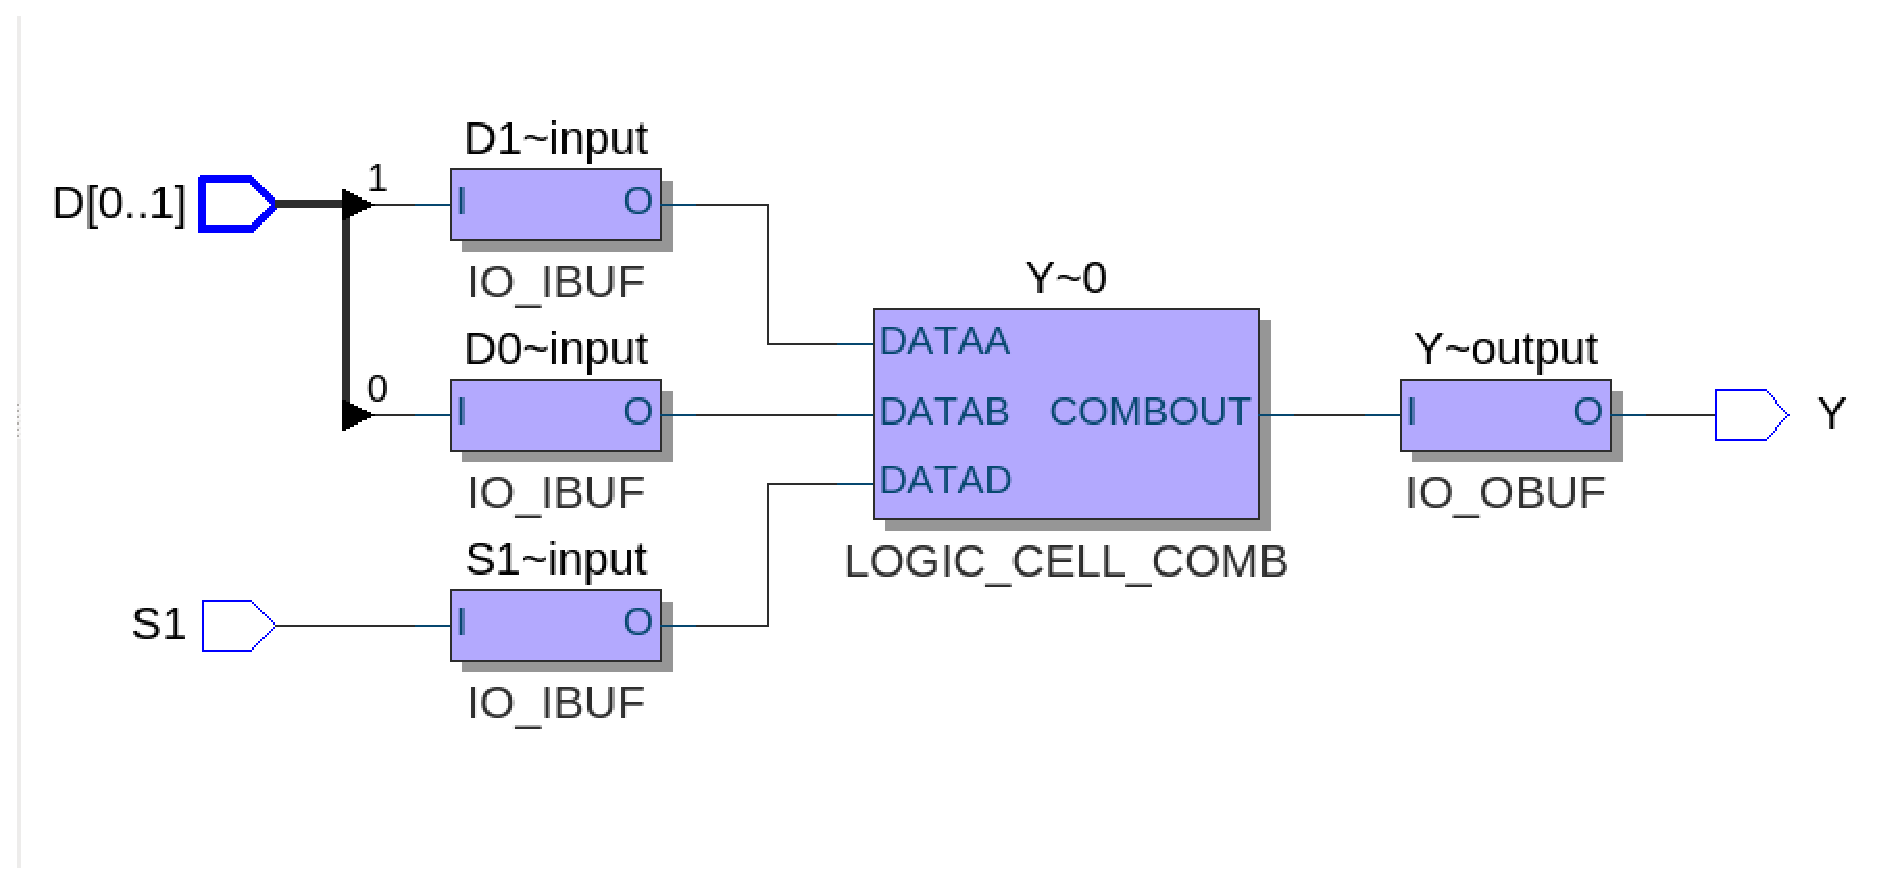
\includegraphics[width=13cm]{images/fig03.eps}
    \caption{最適化後の回路構成}
    \label{fig:03}
  \end{center}
\end{figure}

コンパイル結果のロジックエレメント数は図\ref{fig:04}のようだった. 
ロジックエレメント数は図\ref{fig:04}のTotal Logic Elementの部分である。

\begin{figure}[htb]
  \begin{center}
    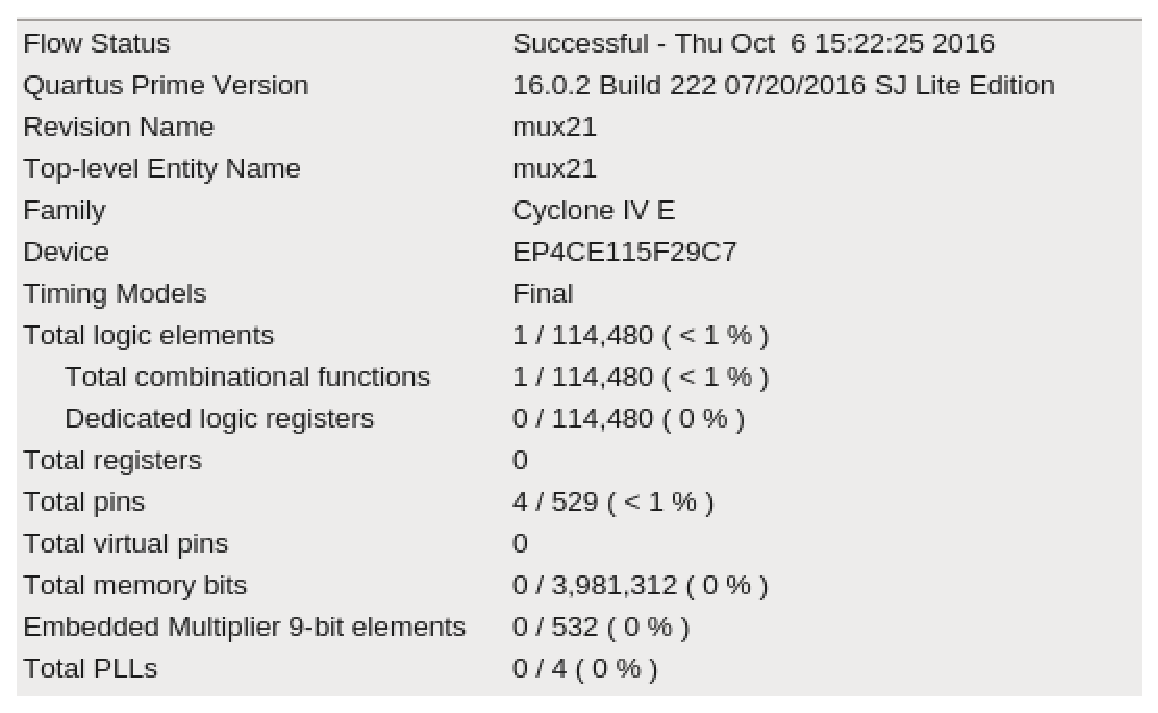
\includegraphics[width=10cm]{images/fig04.eps}
    \caption{ロジックエレメント数}
    \label{fig:04}
  \end{center}
\end{figure}

回路の遅延時間は図\ref{fig:05}の通りだった.
トータルの遅延時間はここでは、13.447nsとなる。

\begin{figure}[htb]
  \begin{center}
    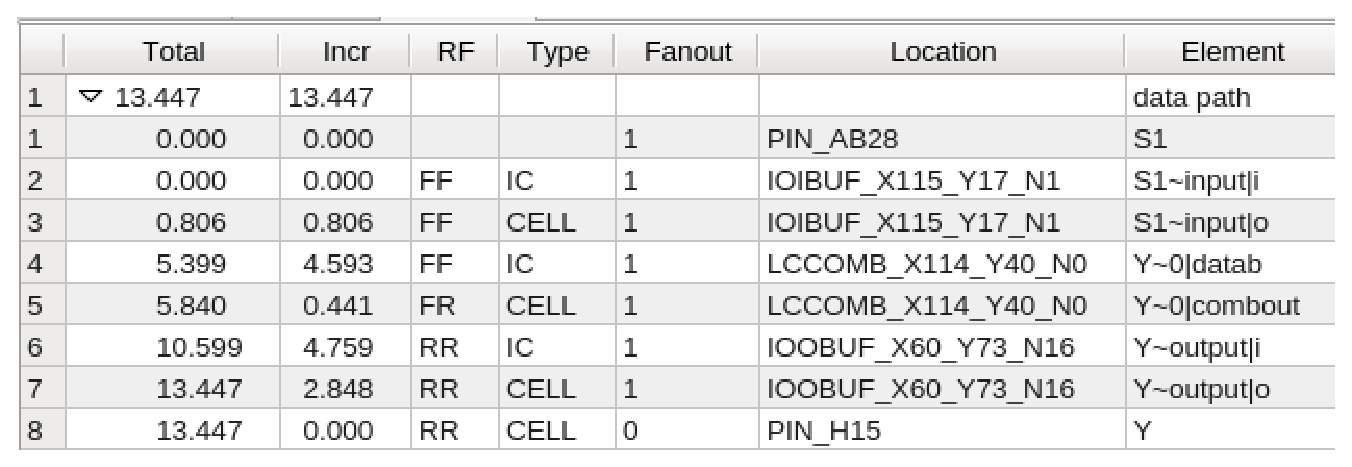
\includegraphics[width=10cm]{images/fig05.eps}
    \caption{遅延時間}
    \label{fig:05}
  \end{center}
\end{figure}

%----------------------------------
\subsubsection{FPGAボードでの動作実験}
%----------------------------------

表\ref{tab:1}で示したものと同じ結果になった.

\clearpage

%---------------------------------------------------------------------
\subsection{考察}
%---------------------------------------------------------------------

%----------------------------------
\subsubsection{機能レベルシミュレーション結果に対する評価}
%----------------------------------

図\ref{fig:02}の波形は、入力した値から、0の時は波形の下方、1の時は波形の情報で示されていることが推察される。
図\ref{fig:02}の{\tt /test\_mux21/Y}の波形に注目すると、表\ref{tab:1}で予想したYの出力値と一致している。
\bou{テストパターンに大して}、論理式$(\lnot S_1 \land D_0) \lor (S_1 \land D_1)$による出力が正確に行われている事が検証できたと言える。

%----------------------------------
\subsubsection{テストパターンは適切だったか}
%----------------------------------

今回のテストパターンは(S_1, D_0, D_1)が(0, 0, 0), (0, 1, 0), (1, 1, 0)の場合しか検証をしていない。これは1ビットの入力が3つある今回の状況
においては全てもパターンを網羅しているとは言えない。実際にS1がボタンに対応しているので、現実にそったテストパターンを考えると以下がよいだろう。

\begin{lstlisting}[basicstyle=\ttfamily\footnotesize, frame=single]


always begin
  # 10 S1 = ~S1;
end

initial begin
  S1 = 0; D0 = 0; D1 = 0;

  # 50 D0 = 0; D1 = 1;
  # 50 D0 = 1; D1 = 0;
  # 50 D0 = 1; D1 = 1;
  # 50 $finish;
end
\end{lstlisting}

このようにすると(D0, D1) = (0, 0), (0, 1), (1, 0), (1, 1)の全てのパターンについて50nsごとにテストして、その間10nsごとにボタン(S1)を押したり押さなかったりを繰り返す
ような人間らしいテストパターンが出来上がった。このテストパターンだと初期のテストで網羅できていなかったパターンも確認できる。

ただし、今回の実験は簡単な例だったが、複雑な論理式になると、少ないパターンでの検証は不適切であると考えられる。

%----------------------------------
\subsubsection{回路構成とロジックエレメント数の関係}
%----------------------------------

回路構成とロジックエレメント数の関係を考察するには、 Total logic elements に含まされる Total combinational functions(組み合わせ関数) と Dedicated logic registers(論理レジスタ)の定義を知る必要がある。

文献\cite{et01}では、Combinational Logic Circuits(組み合わせ論理回路)を「入力値に対する出力値がメモリの順序に依存する順序論理回路とは異なり、組み合わせ論理回路は論理関数により、入力値に対して出力値が即座に決定される」と説明している。
Dedicated logic registersはこの実験では0なので、現れた実験で考察を加えることにする。

上記の例は簡単にまとめると、今回の実験は回路の状態を保持せず、与えられた入力値に対して即座に出力が決まるということだと考えられる。

図\ref{fig:03}の最適化後の回路構成を見ると、 {\tt Y-0}と囲まれたブロックが、以上の組み合わせ論理回路の定義を満たしていることが分かる。

Flow Summaryに示されているTotal combinational functionsは最適化後の回路構成における組み合わせ論理回路の総数を表していることが実験結果から推察できる。


\clearpage


%===================================================================
\section{加算を行う組み合わせ回路の設計(実験2)}
%===================================================================

%---------------------------------------------------------------------
\subsection{目的・概要}
%---------------------------------------------------------------------

今回の実験では、VerilogHDLを用いて16ビット加算回路の設計を行う。
16ビット加算回路は計算式の $sum = x + y$ のような加算を行い、今回用いる変数は
どちらも16ビットなので、 $2~{16} = 65536$ までの演算が可能である。

VerilogHDLで回路を記述した後は、前回の実験と同様にテストベンチを用いて、16ビット加算器として適切な動作をしているかを確認する。
なお、今回の実験ではFPGAでの実験は行わない。

%---------------------------------------------------------------------
\subsection{実験手順}
%---------------------------------------------------------------------

今回の実験では、16ビット加算回路の設計を行った。今回作成する回路の仕様は以下の通りである。

\begin{itemize}
  \item 入力: 被演算数x, y(各16ビット), 桁上げ入力cin(1ビット)
  \item 出力: 和sum(16ビット)、桁上げ出力cout(1ビット)
  \item 機能: x + yを計算し、和と桁上げを出力する組み合わせ回路
\end{itemize}

はじめに、この16ビット加算回路をVerilogHDLで記述した。そのコードは以下の通りである。


\lstinputlisting[caption=セレクタ回路のテストベンチ,label=test_mux21.v]{../../jikken2/adder16.v}

このコードの構造を説明する。

\begin{itemize}
  \item 1~4行目はコメントである。
  \item 6行目で今回の回路のモジュール「{\tt adder16}」を宣言している。
  \item 7行目で16ビットの入力としてx, yを宣言した。今回作成する加算器は16ビット仕様なので、16ビット幅のポートx, yを持つ必要があり、
          そのために、{\tt [15:0]}としている。
  \item 8行目で桁上げ用に1ビットの入力cinを宣言した。
  \item 10行目で計算結果を出力するために16ビットのsumを宣言した。
  \item 11目目で桁上げ用の出力として1ビットのcoutを宣言した。
  \item 13行目で回路本体の加算部分の記述をした。
        {\tt \{cout, sum\}}で2つのオペランドを1つのビット表現にまとめているので、17ビット長の変数となっている。ここに$x + y + cin$の結果が入る。
	  この時に、桁上げがあれば、16ビットから繰り上がって17ビット目が1になるので、結果として出力用の桁上げ出力が1となる。
\end{itemize}

次に、16ビット加算回路のテストベンチを作成した。そのコードは以下の通り。

\lstinputlisting[caption=セレクタ回路のテストベンチ,label=test_mux21.v]{../../jikken2/test_adder16.v}

同様にこのコードの構造を説明する。

\begin{itemize}
  \item 1~4行目はコメントである。
  \item 6行目で {\tt assign}文における時間の単位を{\tt `timescale}によって指定している。
  \item 7行目で上で記述した16ビット加算回路の本体を取り込んでいる。
  \item 9行目以降で、{\tt test}モジュールを定義している。
  \item 10行目で、テストパターンを与える対象として{\tt x, y}を宣言した。
  \item 11行目で、テストパターンを与える対象として{\tt cin}を宣言した。
  \item 13行目で、信号を観測する対象として、{\tt sum}を宣言した。
  \item 14行目で、信号を観測する対象として、{\tt cout}を宣言した。
  \item 16行目で、{\tt adder16)を実体化した。
  \item {\tt always}ブロックのオブジェクトの値に変化が生じた場合に、シミュレータのブロック内の手続きを一回実行して、次のイベントが発生するのを待つ。
           そのため、18行目で{\tt x}に変化が生じたときに、10nsの遅延でこの演算が行われる。結果的にこの演算は再帰的に実行されることになるので、xは10nsごとに
           100ずつ加算されていくことを意味する。
  \item 22行目も同様に毎回5nsの遅延で演算を再帰的に繰り返すため、5nsごとにyに300が加算されていく。
  \item 26行目の{\tt initial}ブロックは、ブロック内の処理を一回実行するだけで終了するため、{\tt x, y, cin}に初期値を設定している。
\end{itemize}















//ここかラマ高く



















次に,機能レベルシミュレーション,論理合成を行った.
実験の手続きは,実験1と同様なので省略する.

\subsection{実験結果}

\subsubsection{機能レベルシミュレーション}

図\ref{fig:09}に示す波形を得た.

\begin{figure}[htb]
  \begin{center}
    \includegraphics[width=13cm]{images/fig-09.eps}
    \caption{機能レベルシミュレーションを行った結果の波形}
    \label{fig:09}
  \end{center}
\end{figure}

\subsubsection{論理合成}

最適化後の回路構成は,図\ref{fig:lb-01}(巻末に掲載)のようになった.

コンパイル結果のロジックエレメント数は図\ref{fig:11}のようだった. 

\begin{figure}[htb]
  \begin{center}
    \includegraphics[width=10cm]{images/fig-11.eps}
    \caption{ロジックエレメント数(点線で囲んだ箇所)}
    \label{fig:11}
  \end{center}
\end{figure}

回路の遅延時間は図\ref{fig:10}の通りだった.

\begin{figure}[htb]
  \begin{center}
    \includegraphics[width=10cm]{images/fig-10.eps}
    \caption{遅延時間(点線で囲んだ箇所)}
    \label{fig:10}
  \end{center}
\end{figure}

\subsection{考察}

\subsubsection{機能レベルシミュレーション結果に対する評価}

図\ref{fig:09}から,期待通りに加算が行われていることが分かる.
ある時間軸上の {\tt sum} の値が,同じ時間軸上にある {\tt x, y} の和になっている.

\subsubsection{回路構成とロジックエレメント数の関係の検討}

実験結果の回路構成はやや膨大であり,その仕組みを検討するのが困難であるので,まずは,一般的な4ビット加算機の論理回路を確認することにする.
図\ref{fig:13}のように,桁上げ入力 {\tt ci}と入力 {\tt a, b} が各全加算機(Full Adder: FA)に入力されている.
一方,各全加算機からは,出力値 {\tt s} と桁上げ出力 {\tt w} が出力されている.
{\tt s} が加算の結果となる.

\begin{figure}[htb]
  \begin{center}
    \includegraphics[width=6cm]{images/fig-13.eps}
    \caption{4ビット加算機の論理回路図(文献\cite{hdl}を参考に作成)}
    \label{fig:13}
  \end{center}
\end{figure}

4ビット加算機の仕組みをもとに考えてみると,16ビット加算機の回路構成についても,同様の仕組みであることが分かる.

\begin{figure}[htb]
  \begin{center}
    \includegraphics[width=13cm]{images/fig-14.eps}
    \caption{16ビット加算機の入出力と桁上げ入力}
    \label{fig:14}
  \end{center}
\end{figure}

\begin{figure}[htb]
  \begin{center}
    \includegraphics[width=7cm]{images/fig-15.eps}
    \caption{16ビット加算機の入出力と桁上げ出力}
    \label{fig:15}
  \end{center}
\end{figure}

4ビット加算機で示した,全加算機と入力および桁上げ入力にあたる箇所を図\ref{fig:14}に示した.
また,出力および桁上げ出力に関しても,同様の回路構成をとっていることが分かる(図\ref{fig:15}).
加算機の入出力付近を検討したが,その間の全加算機についても,4ビット加算機と同様の入出力がされていると推測できる.

16ビット加算機において,全加算機がロジックエレメントの最小単位であると推察できる.
しかし,ロジックエレメントの数は18であると示されていた.
{\tt cin, cout}と全加算機の間にある,空のブロックがこのロジックエレメントに含まれていると仮説を立てると,示された数と合う.
2〜15番目の全加算機の桁上げ入出力によって繋がれている前後がロジックエレメントであるから,1, 16番目も同様にロジックエレメントに接続されたと推察した.
空のロジックエレメントが生じた具体的な原因は突き止めることができなかった.

\clearpage

\section{加算を行う順序回路の設計(実験3)}

\subsection{目的・概要}

本実験では,16ビット加算機を順序回路で設計する.

前節でも少し触れたが順序回路について定義を確認したい.
順序回路は,出力が過去の入力にも依存する論理回路である.
順序回路は,組み合わせ回路部分と記憶回路部分で表現される.
記憶回路部分は組み合わせ回路回路からの出力を記憶し,記憶された状態は組み合わせ回路部分への次の入力となる.
入力は時間とともに変化するが,クロックパルスに同期して規則正しい時間間隔で入力を変化させる同期式と,そうでない非同期式がある.



\subsection{実験手順}

本実験では,16ビット加算回路の設計を行った.
仕様は以下の通りであった.

\begin{itemize}
  \item 入力: 被演算数x, y(各16ビット),桁上げ入力cin(1ビット)
  \item 出力: 和sum(16ビット),桁上げ出力cout(1ビット)
  \item 機能: x+yを計算し,和と桁上げを出力する組み合わせ回路
\end{itemize}

まず,Verilog HDLで回路記述を行った.
16ビット加算回路の構造を説明する.

\begin{itemize}
  \item 
    7〜10行目で入出力を設定した.
    実験2と異なるのは,入力として {\tt clk, reset} が追加されている点である.
  \item 
    12行目で現在の値を記憶しておくflip-flop(16bitレジスタ) {\tt r0, r1}の宣言ををした.
  \item 14行目で,出力ポートへの代入を行った.
  \item 
    16行目以降で処理を記述した.
    {\tt always}が発生する条件として,クロックの立ち上げり {\tt (posedge clk: positive edge click)}とリセット信号の立ち下がり {\tt (negedge reset: negative edge reset)}検出している.
  \item 
    18, 19行目で, {\tt reset == 0},つまり {\tt reset} バイナリの1桁目が0のとき, {\tt r0, r1}のリセットする制御を記述した.
    {\tt <=}で書かれる代入は,ノンブロッキング代入と呼ばれ, {\tt begin - end}内の右辺の評価がすべて行われた後,すべての代入が同時に実行される.
  \item
    20〜23行目で,{\tt reset != 0},つまり {\tt reset} バイナリの1桁目が1のとき, {\tt r0}を {\tt x} の値に, {\tt r1}を {\tt y}の値にする制御を記述した.
\end{itemize}

次に,16ビット加算回路のテストベンチを作成した.

\begin{itemize}
  \item 
    8行目で16ビット加算機の読み込みを行った.
  \item 
    10行目以降で, {\tt test}モジュールを宣言している.
  \item 
    11, 12行目で,信号を与える入力ポートを与えた.
  \item 
<<<<<<< HEAD
    14, 15行目で,信号を観測する対象のポートを与えた.s
=======
    14, 15行目で,信号を観測する対象のポートを与えた.
  \item
    17行目で,16ビット加算機の実体化する処理を記述した.
  \item
    19〜21行目で,クリック信号を出力する処理を記述した.
    5ns毎に {\tt clk} がビット反転するようにした.
  \item
    23〜26行目で,演算の対象となる2つの数字を記述した.
    加算が行われていることを確かめる方法として, {\tt x} と {\tt y} の値が増えていき,その値に対して加算が正確に行われているかどうかを確かめることを試みた.
  \item
    28〜33行目で,初期値の設定を行った.
    31, 32行目ではリセット信号の挙動を確かめるために,処理開始後20秒まで {\tt 1} に,その後 20 秒間 {\tt 0} になった後,また元に戻る処理をした.  
>>>>>>> origin/master
\end{itemize}

次に,機能レベルシミュレーション,論理合成を行った.
実験の手続きは,実験1と同様なので省略する.

\subsection{実験結果}

\subsubsection{機能レベルシミュレーション}

図\ref{fig:3-01}に示す波形を得た.

\begin{figure}[htb]
  \begin{center}
    \includegraphics[width=13cm]{images/fig3-01.eps}
    \caption{機能レベルシミュレーションを行った結果の波形}
    \label{fig:3-01}
  \end{center}
\end{figure}

\subsubsection{論理合成}

最適化後の回路構成は,図\ref{fig:lb-01}(巻末に掲載)のようになった.

コンパイル結果のロジックエレメント数は図\ref{fig:3-02}のようだった. 

\begin{figure}[htb]
  \begin{center}
    \includegraphics[width=10cm]{images/fig3-02.eps}
    \caption{ロジックエレメント数(点線で囲んだ箇所)}
    \label{fig:3-02}
  \end{center}
\end{figure}

回路の遅延時間は図\ref{fig:3-03}の通りだった.

\begin{figure}[htb]
  \begin{center}
    \includegraphics[width=10cm]{images/fig3-03.eps}
    \caption{遅延時間(点線で囲んだ箇所)}
    \label{fig:3-03}
  \end{center}
\end{figure}

\subsection{考察}



\clearpage

\section{1桁BCDカウンタの設計(実験課題1)}

\subsection{目的・概要}

\subsection{実験手順}

まず,Verilog HDLで回路記述を行った.
1桁BCDカウンタの構造を説明する.

\begin{itemize}
  \item 6行目から,BCDカウンタのモジュールブロックを記述した.
  \item 7, 8行目で,入出力を記述した.
  \item 10行目で,4-bit レジスタを設定した.
  \item 12行目で,出力 {\tt bcd1\_out} にレジスタの値 {\tt count\_reg}を代入した.
  \item 
    14行目から, {\tt always}ブロックの記述をした.
    {\tt always}が発生する条件として,クロックの立ち上げりとリセット信号の立ち下がり検出している.
  \item 
    15行目の条件分岐では, {\tt reset} の値によって振り分ける.
  \item
    {\tt reset == 1} のとき,リセットする動作をする.
    具体的には,4-bit レジスタの値を {\tt 0} にする.
  \item
    一方, {\tt reset == 0} のとき,さらに {\tt x == 1} のとき,カウンタが動く動作をする.
    カウンタでは, {\tt count\_reg} が {\tt 1001}(10進数で {\tt 9})のとき,レジスタの値を {\tt 0}にする.
    それ以外のときは, {\tt count\_reg}をカウントアップ(1を加算)する.
    以上の処理を施した.
\end{itemize}

次に,1桁BCDカウンタを動かすためのテストベンチを作成した.

\begin{itemize}
  \item 6行目で,シミュレーションの単位時間および精度を記述した.
  \item 8行目で,bcd1.v を読み込んだ.
  \item 10行目から,モジュールブロックを開始する.
  \item 12行目で,bcd1 の入力値を格納するレジスタを設定した.
  \item 15行目で,出力を観測するための信号線 {\tt bcd1\_out} を設定した.
  \item 18行目で,bcd1を実体化する処理を記述した.
  \item 20〜23行目で,5ns毎にクリック信号を送る記述をした. {\tt clk} を反転することでこれを実現している.
  \item 24〜26行目で,15ns毎に {\tt x} を有効に,つまりカウンタを動かすようにする処理を設定した.
  \item 
    28行目からは,初期値の設定をした.
    {\tt reset} に関して,最初は {\tt 1},20ns後に一度値を {\tt 0} にした後,さらに20ns後に {\tt 1}に戻した.
    また,さらに1000ns後にテストベンチを終了する記述をした.  
\end{itemize}

\subsection{実験結果}

\subsubsection{機能レベルシミュレーション}

図\ref{fig:4-01}に示す波形を得た.

\begin{figure}[htb]
  \begin{center}
    \includegraphics[width=13cm]{images/fig4-01.eps}
    \caption{機能レベルシミュレーションを行った結果の波形}
    \label{fig:4-01}
  \end{center}
\end{figure}

\subsubsection{論理合成}

最適化後の回路構成は,図\ref{fig:lb-01}(巻末に掲載)のようになった.

コンパイル結果のロジックエレメント数は図\ref{fig:4-02}のようだった. 

\begin{figure}[htb]
  \begin{center}
    \includegraphics[width=10cm]{images/fig4-02.eps}
    \caption{ロジックエレメント数(点線で囲んだ箇所)}
    \label{fig:4-02}
  \end{center}
\end{figure}

回路の遅延時間は図\ref{fig:4-03}の通りだった.

\begin{figure}[htb]
  \begin{center}
    \includegraphics[width=10cm]{images/fig4-03.eps}
    \caption{遅延時間(点線で囲んだ箇所)}
    \label{fig:4-03}
  \end{center}
\end{figure}

\subsection{考察}

\clearpage

\section{2桁BCDカウンタの階層設計(実験課題1)}

\subsection{目的・概要}

\subsection{実験手順}

まず,Verilog HDLで回路記述を行った.
2桁BCDカウンタの構造を説明する.

\begin{itemize}
  \item 1行目で,bcd1.vを読み込む記述を行った.
  \item 3行目から, {\tt bcd2}のモジュールブロックを記述した.
  \item 4, 5行目で入出力を設定した.
  \item 8〜11, 14〜17行目では,出力を観測するための信号線を設定した.
  \item 20, 21行目で,入力のクリック信号を {\tt bcd1a, bcd1b} へ送る記述をした.
  \item 24, 25行目で,入力のリセット信号を {\tt bcd1a, bcd1b} へ送る記述をした.
  \item 28行目で,入力の {\tt x} のレベルを {\tt bcd1a} へ送る記述を行った.
  \item 
    31, 32行目で, {\tt bcd1a, bcd1b} の実体化を行った.
    {\tt bcd1a\_clk}はクリック信号, {\tt bcd1a\_reset}はリセット信号, {\tt bcd1a\_x} は {\tt x} を入力として与えており, {\tt bcd1a\_out} で4bit出力を得ている.
    {\tt bcd1b}についても同様である.
  \item 
    35行目で,2桁目のカウントアップ信号を制御する記述を行った.
    1桁目が9のとき,かつ, {\tt x}が1のとき,二桁目がカウントされる.
    つまり {\tt bcd1b\_x} に与える {\tt x} が1になればよいので, {\tt bcd1a\_out}が {\tt 1001}かつ, {\tt x} を論理式で与えた.
  \item
    28行目で,2桁BCDカウンタの出力を行った.
\end{itemize}

次に,2桁BCDカウンタを動かすためのテストベンチを作成した.
1桁BCDカウンタと動作の仕組みは同様なので,プログラムの説明は省略する.

\subsection{実験結果}

\subsubsection{機能レベルシミュレーション}

図\ref{fig:4-04}に示す波形を得た.

\begin{figure}[htb]
  \begin{center}
    \includegraphics[width=13cm]{images/fig4-04.eps}
    \caption{機能レベルシミュレーションを行った結果の波形}
    \label{fig:4-04}
  \end{center}
\end{figure}

\subsubsection{論理合成}

最適化後の回路構成は,図\ref{fig:lb-02}(巻末に掲載)のようになった.

コンパイル結果のロジックエレメント数は図\ref{fig:4-05}のようだった. 

\begin{figure}[htb]
  \begin{center}
    \includegraphics[width=10cm]{images/fig4-05.eps}
    \caption{ロジックエレメント数(点線で囲んだ箇所)}
    \label{fig:4-05}
  \end{center}
\end{figure}

回路の遅延時間は図\ref{fig:4-06}の通りだった.

\begin{figure}[htb]
  \begin{center}
    \includegraphics[width=10cm]{images/fig4-06.eps}
    \caption{遅延時間(点線で囲んだ箇所)}
    \label{fig:4-06}
  \end{center}
\end{figure}


\subsection{考察}

\clearpage

\section{系列検出回路の設計(実験課題2)}

\subsection{目的・概要}

\subsection{実験手順}

Verilog HDLで回路記述を行った.
系列検出回路の構造を説明する.

\begin{itemize}
  \item 1〜4行目で,4つの状態の値を定義した.st0, st1, st2, st3 の順に二進数で 00, 01, 10, 11 とした.
  \item 6行目からモジュールブロックを記述した.
  \item 7, 8行目で,入出力を設定した.
  \item 10行目で,出力値を収める 1-bit レジスタを設定した.
  \item 11行目で,状態を記憶しておく 2-bit レジスタを設定した.
  \item 13行目で,出力 {\tt y} に出力レジスタの値を代入した.
  \item 
    15行目から, {\tt always}ブロックの記述をした.
    {\tt always}が発生する条件として,クロックの立ち上げりとリセット信号の立ち下がり検出している.
  \item 18, 19行目で, {\tt reset} が {\tt 1} のとき,つまり,リセット信号を検出している際にレジスタが初期化されるように設定した.
  \item 
    21〜57行目では,状態遷移の本体となる記述を行った.
    状態はレジスタ {\tt st\_reg} に記録されており,その値によって {\tt case} 構文により分岐した.それぞれの状態において,入力値を条件分岐により,レジスタ {\tt st\_reg, y\_reg} を状態遷移図にあわせて設定した.
\end{itemize}

次に,系列検出回路を動かすためのテストベンチtest\_mv.vを作成した.

\begin{itemize}
  \item 6行目で,シミュレーションの単位時間および精度を記述した.
  \item 8行目で,m.v を読み込んだ.
  \item 10行目から,モジュールブロックを開始した.
  \item 12行目で,m の入力値を格納するレジスタを設定した.
  \item 15行目で,出力を観測するための信号線 {\tt y} を設定した.
  \item 18行目で,m を実体化する処理を記述した.
  \item 20〜23行目で,5ns毎にクリック信号を送る記述をした. {\tt clk} を反転することでこれを実現している.
  \item
    24〜46行目では,テスト本体を記述した.
    まず,初期値を設定した.
    リセット信号に関しては,はじめの20nsは {\tt 1} に,次の20nsは {\tt 0} に,さらに20ns後に1に戻る設定をした.
    次に,系列 {\tt 1001110010} を順次印加した.
    また,さらに1000ns後にテストベンチを終了する記述をした. 
\end{itemize}

\subsection{実験結果}

\subsubsection{機能レベルシミュレーション}

図\ref{fig:5-01}に示す波形を得た.

\begin{figure}[htb]
  \begin{center}
    \includegraphics[width=13cm]{images/fig5-01.eps}
    \caption{機能レベルシミュレーションを行った結果の波形}
    \label{fig:5-01}
  \end{center}
\end{figure}

\subsubsection{論理合成}

最適化後の回路構成は,図\ref{fig:5-04}(巻末に掲載)のようになった.

\begin{figure}[htb]
  \begin{center}
    \includegraphics[width=13cm]{images/fig5-04.eps}
    \caption{最適化後の回路構成}
    \label{fig:5-04}
  \end{center}
\end{figure}

コンパイル結果のロジックエレメント数は図\ref{fig:5-02}のようだった. 

\begin{figure}[htb]
  \begin{center}
    \includegraphics[width=10cm]{images/fig5-02.eps}
    \caption{ロジックエレメント数(点線で囲んだ箇所)}
    \label{fig:5-02}
  \end{center}
\end{figure}

回路の遅延時間は図\ref{fig:5-03}の通りだった.

\begin{figure}[htb]
  \begin{center}
    \includegraphics[width=10cm]{images/fig5-03.eps}
    \caption{遅延時間(点線で囲んだ箇所)}
    \label{fig:5-03}
  \end{center}
\end{figure}



\subsection{考察}

\clearpage

\section{論理回路の最適化について}

この節では主に,参考文献\cite{siba}を参考に記述している.

\subsection{最適化の目的と指針}

論理回路の最適化が必要な理由は「論理回路を論理ゲートや配線という基本部品によって構成する」からである.
論理ゲートの個数が減り,配線が簡単になると以下のようなメリットがある.

\begin{enumerate}
  \item 論理回路の実装コストが安くなる.
  \item 論理回路の耐故障性が増す.
\end{enumerate}

論理ゲートを論理回路の構成用部品として用いるには,必要な空間や時間の大きさに配慮した設計が必要となる.
論理回路の最適化設計に対する指標は次の2種類がある.

\begin{description}
 \item[空間最適化]\mbox{}\\
   論理回路を構成するのに必要なゲートの総数を最小にする.
 \item[時間最適化]\mbox{}\\
  論理回路の入力端子から出力端子に至までに通過する論理ゲートの段数\footnote{論理回路の入力端子から出力端子に至るまでに通過する論理ゲート数のこと}を最小にする.
  入力端子から出力端子に至るまでの経路は普通複数あるが,時間最適化では,このうち最も多い段数の経路の段数を最小にする.
\end{description}

\subsection{最適化設計の手法}

一般的に,任意の論理関数に対応する論理回路が存在し,逆に,任意の論理回路は論理関数によって表現できることが分かっている.
論理回路図が与えられていて,それをもとにその論理回路を表現する論理関数をもとめることを「論理回路の{\bf 解析}」という.
逆に,論理関数が与えられていて,それをもとにその論理関数に対応する論理回路を求めることを「論理回路の{\bf 解析}あるいは{\bf 合成}」という.

論理回路における論理ゲートは論理関数における論理演算に対応している.
従って,論理ゲートの個数を減らすためには,対応する論理演算の個数を減らせばよい.

最適化設計の手法としては,主に次のようなものが挙げられる.

\begin{description}
 \item[論理関数と論理回路の最小化]\mbox{}\\ 
  論理関数の最適化と論理回路の最適化は連動しているので,論理関数を最小化する.
 \item[カルノー図による2段階論理最小化]\mbox{}\\
  論理関数の表現法の1つであるカルノー図を用いて組み合わせ回路を直感的に最適化設計する.
 \item[クワイン-マクラスキ法による2段階論理最小化]\mbox{}\\
  論理関数の真理値表表現をもとにして,それを併合・簡単化することによって,論理最小化を図る.
 \item[論理式の変形による多段論理最小化]\mbox{}\\
  論理式から共通項をくくり出す操作を行う.
\end{description}

\subsection{最適化された論理回路の遅延時間と面積の関係}

論理合成から所望の回路を出力させるにはHDLを適切に記述する他に,合成される回路の面積や速度といった制約条件が適切でなければならない.
設計する上で考慮しなけらばならない2つの制約を挙げる.

\begin{description}
 \item[エリア制約]\mbox{}\\ 
   回路の面積やゲート数の制約のこと.
 \item[タイミング制約]\mbox{}\\
  クロック周期と回路の出力ポートに対する最大遅延,最小遅延の制約のこと.
\end{description}

この2つの制約にはトレードオフの関係がある(図\ref{fig:03}).

\begin{figure}[htb]
  \begin{center}
    \includegraphics[width=8cm]{images/fig-03.eps}
    \caption{面積とディレイのトレードオフ}
    \label{fig:03}
  \end{center}
\end{figure}

\begin{thebibliography}{99}
\bibitem{hdl} 深山 正幸・北川 章夫・秋田 純一・鈴木 正國 著, 『HDLによるVLSI設計―VerilogHDLとVHDLによるCPU設計― 第2版』,共立出版(2002年)
\bibitem{siba} 柴山 潔 著, 『コンピュータサイエンスで学ぶ 論理回路とその設計』,近代科学社(1999年)
\bibitem{et01} ``Combinational Logic Circuits using Logic Gates'', \url{http://www.electronics-tutorials.ws/combination/comb_1.html}
\end{thebibliography}

\clearpage

\appendix

\begin{figure}[htbp]
  \begin{center}
    \includegraphics[width=15cm]{images/logic-board-01.eps}
    \caption{最適化後の回路構成}
    \label{fig:lb-01}
  \end{center}
\end{figure}

\begin{figure}[htbp]
  \begin{center}
    \includegraphics[width=15cm]{images/logic-board-02.eps}
    \caption{最適化後の回路構成}
    \label{fig:lb-02}
  \end{center}
\end{figure}

\clearpage

\lstinputlisting[caption=セレクタ回路,label=mux21.v]{../exp1/mux21.v}
\lstinputlisting[caption=セレクタ回路用テストベンチ,label=test-mux21.v]{../exp1/test_mux21.v}
\lstinputlisting[caption=プロジェクトファイル,label=mux21.qpf]{../exp1/mux21.qpf}
\lstinputlisting[caption=FPGA設定ファイル,label=mux21.qsf]{../exp1/mux21.qsf}

\lstinputlisting[caption=16ビット加算回路,label=adder16.v]{../exp2/adder16.v}
\lstinputlisting[caption=16ビット加算回路用のテストベンチ,label=test-adder16.v]{../exp2/test_adder16.v}

\lstinputlisting[caption=16ビット加算回路(順序回路),label=adder16s.v]{../exp3/adder16s.v}
\lstinputlisting[caption=16ビット加算回路(順序回路)用のテストベンチ,label=test-adder16s.v]{../exp3/test_adder16s.v}

\lstinputlisting[caption=BCDカウンタ,label=bcd1.v]{../bcd1/bcd1.v}
\lstinputlisting[caption=BCDカウンタ用のテストベンチ,label=test-bcd1.v]{../bcd1/test_bcd1.v}

\lstinputlisting[caption=2桁BCDカウンタ,label=bcd2.v]{../bcd1/bcd2.v}
\lstinputlisting[caption=2桁BCDカウンタ用のテストベンチ,label=test-bcd2.v]{../bcd1/test_bcd2.v}

\lstinputlisting[caption=系列検出回路,label=m.v]{../m/m.v}
\lstinputlisting[caption=系列検出回路用のテストベンチ,label=test-m.v]{../m/test_m.v}



\end{document}


